\subsubsection{48V Speisung}
\label{subsubec:48V Speisung}


Der Motor wird mit einer Spannung von 48V betrieben. Dies ist zugleich auch die höchste verwendete Speisespannung. Um diese Speisung gewährleisten zu können, wird ein fertiges Netzteil gemäss  \textcolor{red}{\textbf{Fachbericht 5}} eingesetzt. Somit entfällt das Schema für diesen Speisungsteil. Ein Anschauungsbild des eingesetzten Netzteils kann in Abbildung \ref{fig:Netzteil_48V} begutachtet werden \cite{aliexpress_us_nodate}.\\

\begin{figure}[h!]
	\centering
	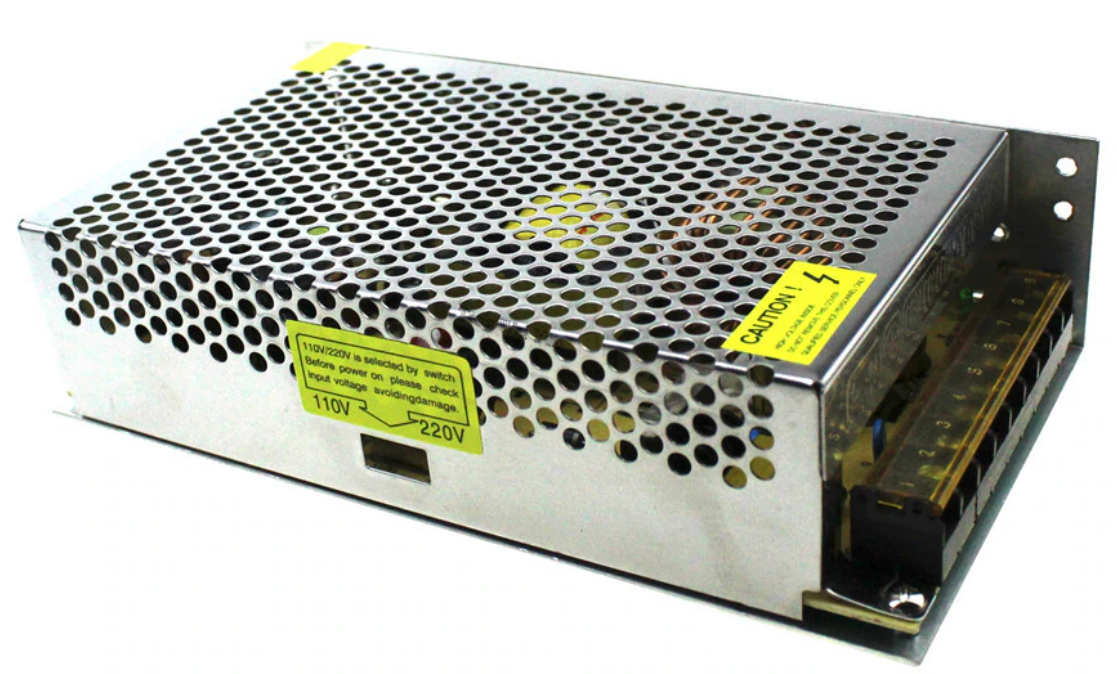
\includegraphics[width=0.5\textwidth]{graphics/Netzteil_48V.png}
	\caption{Anschauungsbild des 48V Netzteils \cite{aliexpress_us_nodate}}
	\label{fig:Netzteil_48V}
\end{figure} 

Eine Leistungsabschätzung war jedoch unabdingbar. Auch diese wurde im Projekt 5 durchgeführt. Unter Berücksichtigung der Schaltungsteile welche noch im Projekt 6 ergänzt werden, wurde dieses dann ausgewählt und eingekauft. Die Leistungsabschätzung kann im \textcolor{red}{\textbf{Fachbericht 5}} eingesehen werden. 

\newpage